\documentclass[tikz,border=2pt]{standalone}
\usepackage{amsmath,amssymb}
\usepackage{tikz}
\usetikzlibrary{matrix}

\begin{document}
% y2 <= y1 ("decision 2 only if decision 1"): of the four yes/no combinations exactly one is
% excluded, namely decision 2 yes while decision 1 is no.
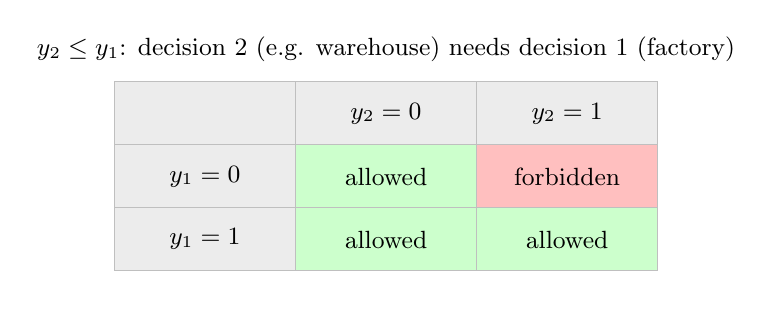
\begin{tikzpicture}[every node/.style={font=\small}]
	\matrix (T) [matrix of nodes, nodes={minimum width=2.3cm, minimum height=8mm, anchor=center, draw=gray!50}, column sep=-\pgflinewidth, row sep=-\pgflinewidth] at (0,0) {
		|[fill=gray!15]| & |[fill=gray!15]| $y_2=0$ & |[fill=gray!15]| $y_2=1$ \\
		|[fill=gray!15]| $y_1=0$ & |[fill=green!20]| allowed & |[fill=red!25]| forbidden \\
		|[fill=gray!15]| $y_1=1$ & |[fill=green!20]| allowed & |[fill=green!20]| allowed \\
	};
	\node[anchor=south] at (T.north) {$y_2\le y_1$: decision 2 (e.g. warehouse) needs decision 1 (factory)};
	\end{tikzpicture}
\end{document}
